\documentclass[conference]{IEEEtran}

% 4 oder 8 Seiten

\IEEEoverridecommandlockouts

\usepackage{cite}
\usepackage[pdftex]{graphicx}

\ifCLASSOPTIONcompsoc
  \usepackage[caption=false,font=normalsize,labelfont=sf,textfont=sf]{subfig}
\else
  \usepackage[caption=false,font=footnotesize]{subfig}

\usepackage[bookmarks=false]{hyperref}

\hyphenation{}

\newcommand{\citep}{\cite}

\begin{document}

\title{Performance Vergleich von Typ 1 und Typ 2 Hypervisoren }

\author
{
\IEEEauthorblockN{
	Colin Jochum, Tom Kleinhapl}
\IEEEauthorblockA{
	FH JOANNEUM -- University of Applied Sciences\\
	Dep. of Applied Computer Sciences\\
	Alte Poststra\ss e 147\\
	8020 Graz, Austria\\
	Supervisor: FH-Prof. Mag. Dr. Robert Singer}
}

\maketitle

\begin{abstract}
text  
\end{abstract}

\IEEEpeerreviewmaketitle

\section{Einleitung}
\label{Einleitung}

Das Ziel dieser Arbeit ist es Performance Unterschiede zwischen Typ 1 und Typ 2 Hypervisoren zu untersuchen, um signifikante Abweichungen ($>$10\%) hinsichtlich CPU-Rechenleistung und Boot Zeit festzustellen. Dafür wurden zwei Mess-Szenarien entworfen und in einer Testumgebung durchgeführt. Im Kapitel der Arbeit werden theoretische Inhalte der Virtualisierung und der Nutzung von Hypervisoren erläutert, anschließend werden die Messungen und deren Ergebnisse dargelegt und interpretiert. Im letzten Kapitel werden mögliche Schlüsse aus den gewonnenen Erkenntnissen gezogen. 

\section{Virtualisierung und Hypervisoren}
\label{Virtualisierung und Hypervisoren}	
In der Informatik wird der Begriff der Virtualisierung primär mit der Virtualisierung von Hardwareressourcen assoziiert. Darunter versteht man die Nachbildung einer reellen Hardwareressource in einem standardisierten virtuellen Abbild mit Hilfe eines Abstraktions-Layers. Diese abstrahierende Schicht, die zwischen Hardware und Applikation, wird als Hypervisor, oder ursprünglich auch Virtual-Machine-Monitor (VMM) bezeichnet. [1] Durch die Abstraktion der zugrunde liegenden Ressourcen in logische, bietet ein Hypervisor eine virtuelle Umgebung für Betriebssysteme. Grundsätzlich müssen Hypervisoren drei wesentliche Aufgaben erfüllen: 
\begin{itemize}
	\item Eine Umgebung schaffen, die mit der physischen Umgebung ident ist. 
	\item Eine Umgebung mit minimalen Rechenleistungskosten bereitstellen. 
	\item Die Kontrolle über die Systemressourcen bewahren. 
\end{itemize}
[4]

Die ursprüngliche Bezeichnung von Hypervisoren als VMM stammt von deren primären Verwendungszweck der kompletten Systemvirtualisierung von Computern, nämlich das Ausführen von komplett voneinander isolierten Gasbeitriebsystemen in virtuellen Maschinen (VM). Die Form der Komplett-Virtualisierung steht auch im Fokus unserer Mess-Szenarien. Im Kontrast dazu gibt es auch die Paravirtualisierung, bei welcher sich mehrere Gasbetriebsysteme einen Kernel teilen. [2] Die Komplettvirtualisierung ermöglicht ebenfalls das Hosten mehrerer Betriebssysteme, allerdings benutzt hier jede Maschine einen eigenen Kernel. Der Hypervisor selbst erfüllt bei der Ressourcenallokation eine ähnliche Rolle wie ein Betriebssystem. Nur kommen Ressourcenanfragen nicht von einzelnen Anwendungen, sondern von einer VM. [1]

\subsection{Typ1 und Typ2 Hypervisoren}
Bei Hypervisoren wird generell zwischen zwei Architekturen unterschieden: Typ-1-Hypervisoren (auch native oder bare-metal Hypervisor) und Typ-2-Hypervisoren (auch hosted Hypervisor). Ein Typ-1 Hypervisor wird auch als nativer oder bare-metal Hypervisor beschrieben, weil dieser direkt auf der Server Hardware läuft, ohne ein darunterliegendes Betriebssystem zu benötigen. Ein typischer Typ-1 Hypervisor ist VMWare ESXi. Der Typ-2 Hypervisor oder auch hosted Hypervisor läuft über einem traditionellen Betriebssystem, dieses wird auch als Host-Betriebssystem bezeichnet. Ein typischer Typ-2 Hypervisor ist VMWare Workstation. Die verschiedenen Architekturen der beiden Hypervisor Typen werden in der Grafik 1 dargestellt. [2], [3] 

\begin{figure}
	\centering
	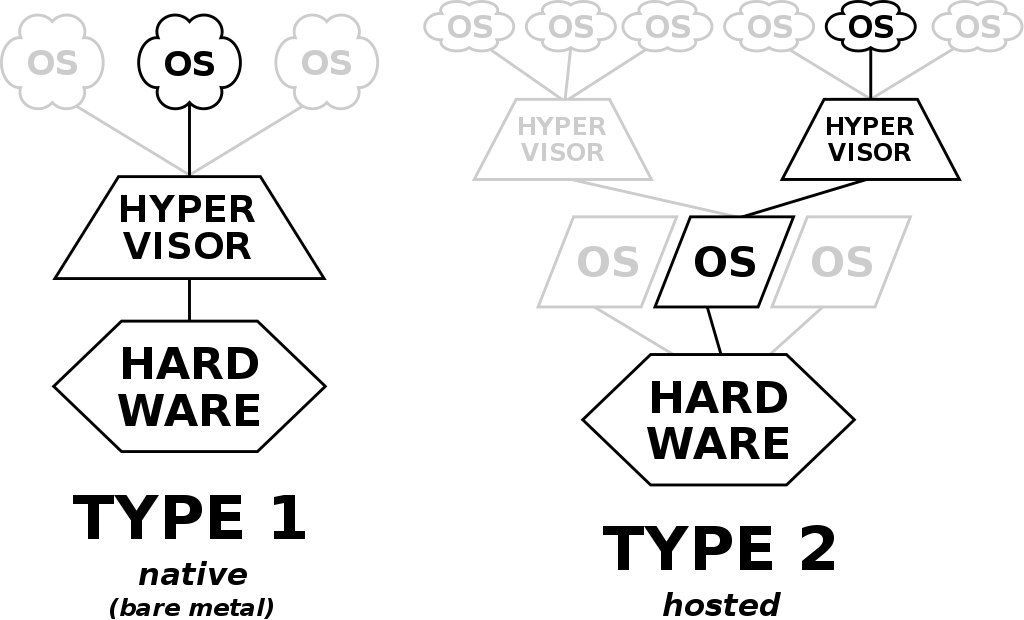
\includegraphics[keepaspectratio,width=8.5cm,height=0.75\textheight]{hypervisors.png}
	\caption{Die Architektur von Typ 1 und Typ 2 Hypervisoren.}
	\label{architecture}
\end{figure}

\section{Computer Spezifikation}
\label{Computer Spezifikation}

\section{Messung der CPU Performance}
\label{Messung der CPU Performance}

\subsection{Messaufbau}

\subsection{Single-Core Performance-Messung}

\subsection{Multi-Core Performance-Messung}

\subsection{Interpretation}

\section{Messung der Boot-Zeit}
\label{Messung der CPU Performance}

\section{Fazit}
\label{Fazit}

\bibliographystyle{IEEEtran}
\bibliography{IEEEabrv,SEAAnew}


\end{document}
